\tikzsetnextfilename{mr_spatial_encoding_2d}
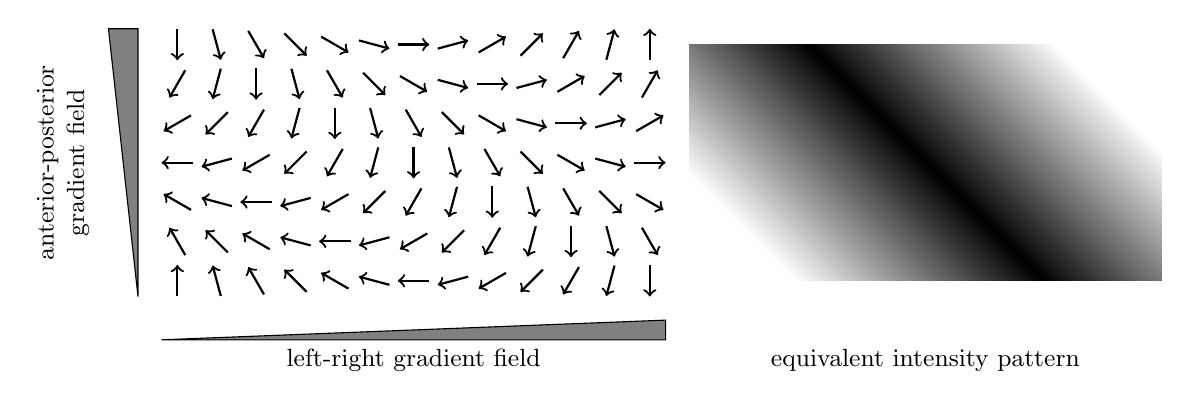
\begin{tikzpicture}[scale=0.5]
	\pgfmathsetmacro{\anglex}{15}
	\pgfmathsetmacro{\angley}{30}
	\pgfmathsetmacro{\startangle}{90}
	\foreach \idx in {0,1,...,12} {
		\foreach \idy in {0,1,...,6} {
			\pgfmathsetmacro{\anglevalue}{\startangle+\idx*\anglex+\idy*\angley}
			\pgfmathsetmacro{\x}{\idx+0.4*cos(\anglevalue)}
			\pgfmathsetmacro{\a}{\idx-0.4*cos(\anglevalue)}
			\pgfmathsetmacro{\y}{\idy+0.4*sin(\anglevalue)}
			\pgfmathsetmacro{\b}{\idy-0.4*sin(\anglevalue)}
			\draw[thick,<-] (\x, \y) -- (\a, \b);
		}
	}
	\begin{scope}[xshift=13cm]
		%\clip (-0.25, 0) rectangle (19.25, 2);
		\fill[left color=white, right color=white, middle color=black, shading angle=135] (0, 0) rectangle (12, 6);
		\coordinate (B) at (6, 3);
	\end{scope}
	\draw[fill=gray] (-0.4, -1.5) -- node (A) [below, font=\small] {left-right gradient field} (12.4, -1.5) -- (12.4, -1.0) -- cycle;
	\draw[fill=gray] (-1, -0.4) -- node [sloped, above=0.5cm, font=\small] {\parbox{3cm}{\centering anterior-posterior \\ gradient field}} (-1, 6.4) -- (-1.75, 6.4) -- cycle;
	\draw (A -| B) node [font=\small] {equivalent intensity pattern};
\end{tikzpicture}